\documentclass[11pt]{article}
\usepackage[a4paper,margin=1in]{geometry}
\usepackage{graphicx,booktabs,longtable,array,amsmath,hyperref}
\hypersetup{hidelinks}
\setlength{\emergencystretch}{1em}
\title{Experimental results: expanded measurement coverage}
\author{}
\date{30 September 2026}
\begin{document}
\maketitle
\noindent This results package covers twenty existing trials. The online proposal must be reconciled with its current source before publication.
\section{Experimental results}
\subsection{Measurement coverage and interpretation}\label{sec:result-metric-coverage}\label{app:four-condition-diagnostics}
Message outcomes use distinct, successfully acknowledged messages produced during evaluation and followed through the end of drain. Completion is recorded after processing, before commit acknowledgment. Warm-up messages are excluded from these outcomes but may contribute to backlog and throughput. Lag, throughput, CPU and memory plots cover evaluation; resource totals cover evaluation plus drain. Missing observations, including during partition handover, remain gaps. The Metrics section defines the calculations, and Appendix~\ref{app:measurement-coverage} lists where each metric is reported.

\clearpage
\subsection{Twelve high-input partitions: ten-minute evaluation}\label{sec:twelve-partition-updated}
The twelve-partition comparison used 700 aggregate messages/s over 60 partitions, with 80\% of traffic directed to twelve partitions initially owned by Consumer 2. Eight trials compared retaining the same three-consumer assignment, redistribution within three, scaling to six with targeted redistribution, and scaling to six with Kafka's normal cooperative rebalance. Each condition was run twice, reversing condition order in the second repetition. Starting ownership and the original consumers' pod identities, nodes and resource declarations were checked before traffic.

Every trial admitted 420,000 evaluation messages. Keeping the initial assignment left 34.64--34.83\% unfinished at cutoff; all interventions completed the cohort. Redistribution within three produced p99 latency of 80.10--84.16 seconds, compared with 100.81--107.24 seconds for targeted scaling and 71.41--72.46 seconds for normal Kafka scaling. The one-second cohort deadline-miss rates reveal a different aspect of the latency distribution: 30.50--31.84\% for redistribution, 26.26--27.33\% for targeted scaling and 21.05--25.83\% for normal scaling, versus 83.32--83.36\% without intervention. Thus a higher p99 does not imply more misses at every deadline.

The resource measurements show the trade-off. Redistribution used approximately 1,035--1,038 observed consumer CPU core-seconds over evaluation plus drain; targeted scaling used 1,310--1,327 and normal scaling 1,452--1,459. Requested CPU was 72 core-minutes for redistribution and approximately 137 for either six-consumer response. Actual RSS integrals were 2.53--2.65, 3.95--4.15 and 3.66--3.69 GiB-minutes respectively. These values concern consumer processes and resource declarations, not total infrastructure cost. The first unchanged baseline lacks almost all local request history and cannot support a full-window request-cost comparison; its message outcomes and recovered historical process measurements remain usable within their stated coverage.

Targeted scaling confirmed recovery sooner than redistribution within three (169.0--184.9 versus 305.2--328.9 seconds after the action decision), despite its higher whole-cohort p99. Recovery requires processing backlog at most 100 offsets for thirty consecutive valid seconds while input continues. Normal scaling's recovery varied from 143.0 to 259.0 seconds. Explicit ownership changes use a global release/acquire/resume barrier; their 14.40--14.54-second and 19.05--19.50-second processing pauses are distinguished from complete action duration. Normal cooperative scaling had much shorter global gaps, which does not imply every partition processed continuously.

Persistent hotspots were present before intervention. In the redistribution and targeted-scaling runs, none remained at any defined snapshot in the final two evaluation minutes. The diagnostic figure also shows that relative skew may rise during successful backlog clearance: the maximum and mean absolute partition lags are then small. Persistence and skew are useful descriptions of concentration, but neither alone establishes overload.

Processing-start mean latency ranged from 7.552 to 160.117 seconds across this block; it remains separate from completion latency. Every trial achieved 700 acknowledged evaluation messages/s. No duplicate completion attempts were detected, so completed-attempt and distinct-completion throughput coincide in these trials. Mean application work is reported below; it excludes evidence-writing and offset-commit overhead.
Observed per-process CPU coverage over evaluation plus drain ranged from 87.50\% to 99.72\%. Coverage uses the complete observation window, including time before additional consumers started; a lower value for a newly started consumer is not automatically a monitoring failure. The integral includes only observed valid process intervals.
\begin{table}[!htbp]
\centering\small
\setlength{\tabcolsep}{3pt}
\renewcommand{\arraystretch}{1.12}
\begin{tabular}{@{}lrrrrr@{}}
\toprule
Response & Run & \shortstack{p99\\(s)} & \shortstack{Unfinished\\(\%)} & \shortstack{Misses $>1$ s\\(\%)} & \shortstack{Useful throughput\\(msg/s)}\\
\midrule
Keep 3 & 1 & 366.64 & 34.641 & 83.32 & 423.23\\
Keep 3 & 2 & 362.79 & 34.828 & 83.36 & 422.62\\
Redistribute 3 & 1 & 80.10 & 0.000 & 30.50 & 727.71\\
Redistribute 3 & 2 & 84.16 & 0.000 & 31.84 & 729.53\\
Targeted scale 6 & 1 & 100.81 & 0.000 & 26.26 & 727.75\\
Targeted scale 6 & 2 & 107.24 & 0.000 & 27.33 & 729.31\\
Kafka scale 6 & 1 & 71.41 & 0.000 & 25.83 & 727.65\\
Kafka scale 6 & 2 & 72.46 & 0.000 & 21.05 & 728.48\\
\bottomrule
\end{tabular}
\caption{Whole evaluation-born cohort through the fixed drain cutoff. Deadline misses include overdue unfinished messages. Useful throughput counts distinct completions during evaluation, including warm-up records completed then; it can exceed the input rate while queued work is cleared.}
\label{tab:twelve-partition-outcomes}
\end{table}
\begin{table}[!htbp]
\centering\small
\setlength{\tabcolsep}{3pt}
\renewcommand{\arraystretch}{1.12}
\begin{tabular}{@{}lrrrrr@{}}
\toprule
Response & Run & \shortstack{Actual CPU\\(core-s)} & \shortstack{Actual RSS\\(GiB-min)} & \shortstack{Requested CPU\\(core-min)} & \shortstack{Requested memory\\(GiB-min)}\\
\midrule
Keep 3 & 1 & 892.9 & 3.24 & --- & ---\\
Keep 3 & 2 & 889.7 & 3.24 & 72.00 & 36.00\\
Redistribute 3 & 1 & 1,035.3 & 2.53 & 72.00 & 36.00\\
Redistribute 3 & 2 & 1,037.9 & 2.65 & 72.00 & 36.00\\
Targeted scale 6 & 1 & 1,310.5 & 4.15 & 136.86 & 68.43\\
Targeted scale 6 & 2 & 1,327.5 & 3.95 & 136.80 & 68.40\\
Kafka scale 6 & 1 & 1,451.5 & 3.66 & 137.15 & 68.58\\
Kafka scale 6 & 2 & 1,459.0 & 3.69 & 137.15 & 68.57\\
\bottomrule
\end{tabular}
\caption{Consumer resources over evaluation plus drain. Actual values integrate observed process CPU and RSS intervals and sum them across consumers. Requested values integrate Kubernetes resource declarations; neither is monetary or whole-cluster cost. A dash denotes unavailable full-window request coverage, not zero cost.}
\label{tab:twelve-partition-resources}
\end{table}
\begin{table}[!htbp]
\centering\small
\setlength{\tabcolsep}{3pt}
\renewcommand{\arraystretch}{1.12}
\begin{tabular}{@{}lrrrrrr@{}}
\toprule
Response & Run & \shortstack{Mean total\\lag} & \shortstack{Peak total\\lag} & \shortstack{Lag coverage\\(\%)} & \shortstack{Peak partition\\lag} & Mean skew\\
\midrule
Keep 3 & 1 & 98,929 & 180,743 & 99.7 & 14,752 & 4.90\\
Keep 3 & 2 & 100,033 & 182,438 & 99.7 & 14,794 & 4.90\\
Redistribute 3 & 1 & 7,837 & 46,048 & 96.3 & 5,536 & 9.92\\
Redistribute 3 & 2 & 8,664 & 47,675 & 96.3 & 5,883 & 10.30\\
Targeted scale 6 & 1 & 8,470 & 55,923 & 95.3 & 5,216 & 9.05\\
Targeted scale 6 & 2 & 9,520 & 60,387 & 95.3 & 5,544 & 9.31\\
Kafka scale 6 & 1 & 6,688 & 38,516 & 98.0 & 4,332 & 10.34\\
Kafka scale 6 & 2 & 5,702 & 40,065 & 98.0 & 4,510 & 8.91\\
\bottomrule
\end{tabular}
\caption{Lag diagnostics during evaluation only, in offsets except skew and coverage. Means use trapezoidal area divided by covered time; peaks are sampled maxima. The time mean of the skew ratio is not the ratio of time-averaged maximum and mean lag. Invalid samples and ownership changes are not bridged.}
\label{tab:twelve-partition-diagnostics}
\end{table}
\begin{table}[!htbp]
\centering\small
\setlength{\tabcolsep}{3pt}
\renewcommand{\arraystretch}{1.12}
\begin{tabular}{@{}lrrrrrr@{}}
\toprule
Response & Run & Mean (s) & p50 (s) & p95 (s) & \shortstack{Mean work\\(ms)} & \shortstack{Observed misses\\$>1$ s (\%)}\\
\midrule
Keep 3 & 1 & 158.994 & 161.677 & 341.123 & 2.613 & 72.41\\
Keep 3 & 2 & 160.120 & 164.185 & 344.752 & 2.614 & 72.45\\
Redistribute 3 & 1 & 11.585 & 0.099 & 62.417 & 1.956 & 33.16\\
Redistribute 3 & 2 & 12.676 & 0.100 & 65.276 & 1.943 & 34.61\\
Targeted scale 6 & 1 & 13.813 & 0.124 & 81.024 & 2.451 & 29.08\\
Targeted scale 6 & 2 & 15.245 & 0.125 & 87.387 & 2.457 & 30.27\\
Kafka scale 6 & 1 & 9.140 & 0.120 & 57.805 & 2.764 & 28.66\\
Kafka scale 6 & 2 & 7.555 & 0.120 & 57.333 & 2.773 & 24.15\\
\bottomrule
\end{tabular}
\caption{Supplementary latency diagnostics. Mean, p50 and p95 use completed evaluation-born messages. Mean work is the local monotonic application-processing duration. Observed violations use completion attempts occurring during evaluation and have a different denominator from the primary admitted-cohort deadline rate.}
\label{tab:twelve-partition-latency-details}
\end{table}
\begin{table}[!htbp]
\centering\small
\setlength{\tabcolsep}{3pt}
\renewcommand{\arraystretch}{1.12}
\begin{tabular}{@{}lrrrrrr@{}}
\toprule
Response & Run & \shortstack{Decision to\\active (s)} & \shortstack{Global gap\\(s)} & \shortstack{Extra pending\\during pause} & \shortstack{Net pending\\during transfer} & \shortstack{Recovery\\(s)}\\
\midrule
Keep 3 & 1 & --- & N/A & N/A & N/A & N/A\\
Keep 3 & 2 & --- & N/A & N/A & N/A & N/A\\
Redistribute 3 & 1 & 25.73 & 14.544 & 10,181 & 6,808 & 305.2\\
Redistribute 3 & 2 & 26.01 & 14.400 & 10,081 & 6,581 & 328.9\\
Targeted scale 6 & 1 & 72.81 & 19.498 & 13,648 & 2,082 & 169.0\\
Targeted scale 6 & 2 & 77.18 & 19.049 & 13,350 & 548 & 184.9\\
Kafka scale 6 & 1 & 31.01 & 0.092 & N/A & -6,777 & 259.0\\
Kafka scale 6 & 2 & 33.01 & 0.202 & N/A & -9,823 & 143.0\\
\bottomrule
\end{tabular}
\caption{Intervention costs. For targeted actions, transfer is release request to verified active ownership; for native scaling it is decision to stable-six-owner confirmation. The latter also defines native decision-to-active. Recovery is confirmation after the actual decision. Global gap measures the longest interval without any consumer processing, not a per-partition downtime. Negative net pending change means processing reduced outstanding work during the measured transition. Dashes denote unavailable or inapplicable values.}
\label{tab:twelve-partition-intervention-cost}
\end{table}
\begin{table}[!htbp]
\centering\small
\setlength{\tabcolsep}{3pt}
\renewcommand{\arraystretch}{1.12}
\begin{tabular}{@{}lrrrrrrr@{}}
\toprule
Response & Run & C0 & C1 & C2 & C3 & C4 & C5\\
\midrule
Keep 3 & 1 & 0 & 0 & 12 & --- & --- & ---\\
Keep 3 & 2 & 0 & 0 & 12 & --- & --- & ---\\
Redistribute 3 & 1 & 4 & 4 & 4 & --- & --- & ---\\
Redistribute 3 & 2 & 4 & 4 & 4 & --- & --- & ---\\
Targeted scale 6 & 1 & 2 & 2 & 2 & 2 & 2 & 2\\
Targeted scale 6 & 2 & 2 & 2 & 2 & 2 & 2 & 2\\
Kafka scale 6 & 1 & 0 & 0 & 2 & 4 & 2 & 4\\
Kafka scale 6 & 2 & 0 & 0 & 2 & 4 & 3 & 3\\
\bottomrule
\end{tabular}
\caption{Final observed numbers of configured high-input partitions per consumer. These are traffic targets, not persistent-hot detector counts. All high-input partitions initially belonged to Consumer 2. A dash means no observed partition ownership.}
\label{tab:twelve-partition-ownership}
\end{table}
\begin{table}[!htbp]
\centering\small
\setlength{\tabcolsep}{3pt}
\renewcommand{\arraystretch}{1.12}
\begin{tabular}{@{}lrrrrr@{}}
\toprule
Response & Run & Reference event & C3 (s) & C4 (s) & C5 (s)\\
\midrule
Targeted scale 6 & 1 & Replica request & 63.37 & 63.41 & 63.37\\
Targeted scale 6 & 2 & Replica request & 67.20 & 67.12 & 67.23\\
Kafka scale 6 & 1 & Action decision & 9.22 & 16.43 & 14.35\\
Kafka scale 6 & 2 & Action decision & 9.42 & 18.66 & 9.54\\
\bottomrule
\end{tabular}
\caption{Activation delay to the first valid completion on each added consumer. Targeted scaling uses the recorded replica-request event; native scaling uses the action decision because an equivalent replica-request timestamp was not separately recorded. These are not whole-action completion times or pure rebalance delays.}
\label{tab:twelve-partition-activation-delay}
\end{table}
\clearpage
\begin{figure}[p]
\centering
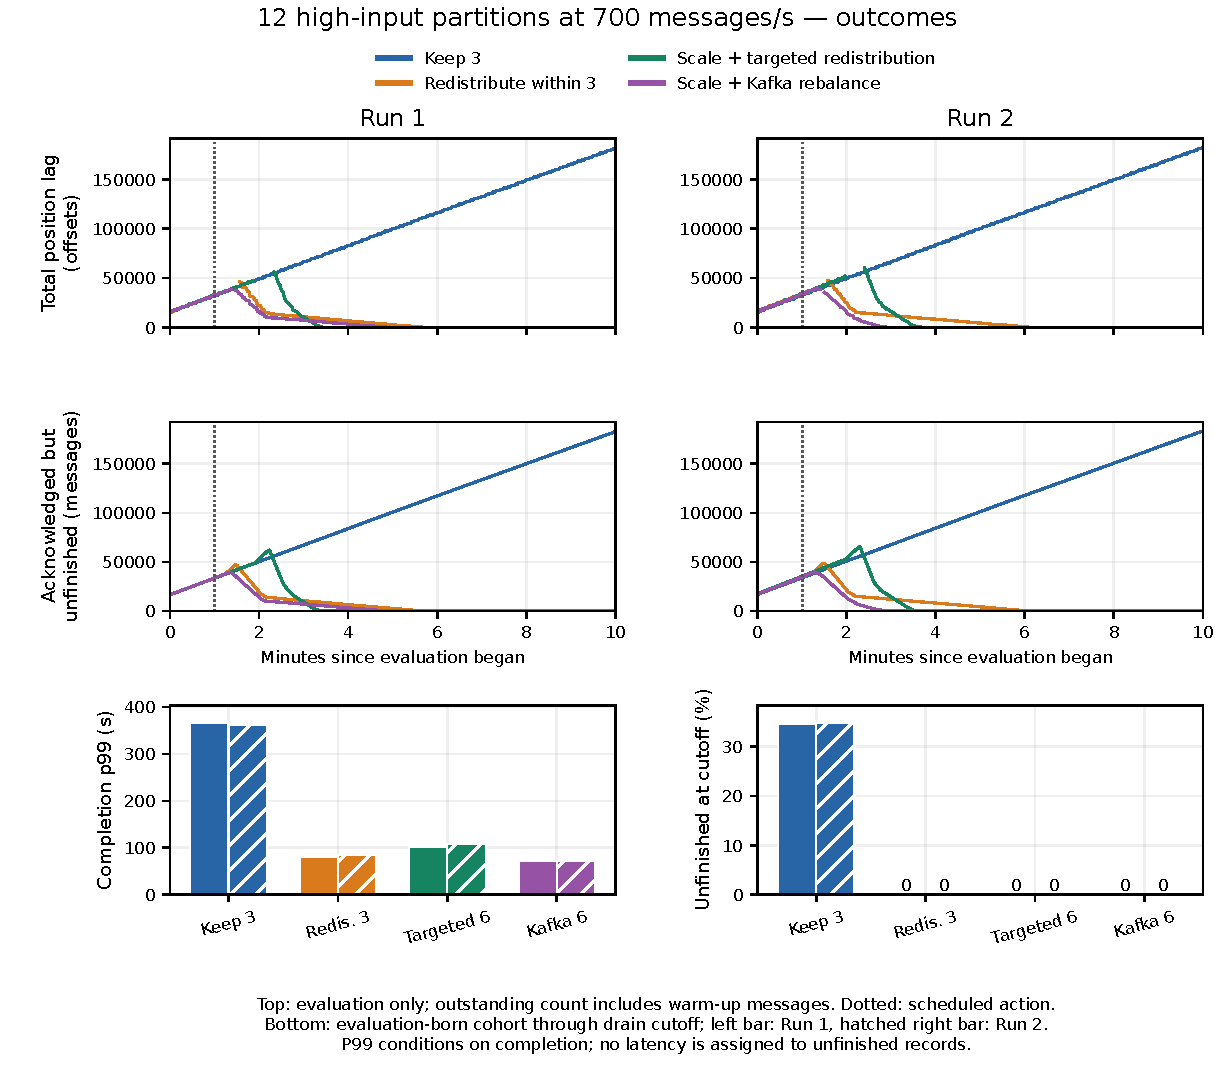
\includegraphics[width=\linewidth,height=.79\textheight,keepaspectratio]{figures/twelve-partition-compact-outcomes.pdf}
\caption{Compact outcome comparison: total consumer-position lag and exact acknowledged-but-unfinished work during evaluation, followed by whole-cohort p99 and unfinished percentage at the drain cutoff. Warm-up work is included in the time-series counts but excluded from the outcome cohort.}
\label{fig:twelve-partition-compact-outcomes}
\end{figure}
\clearpage
\begin{figure}[p]
\centering
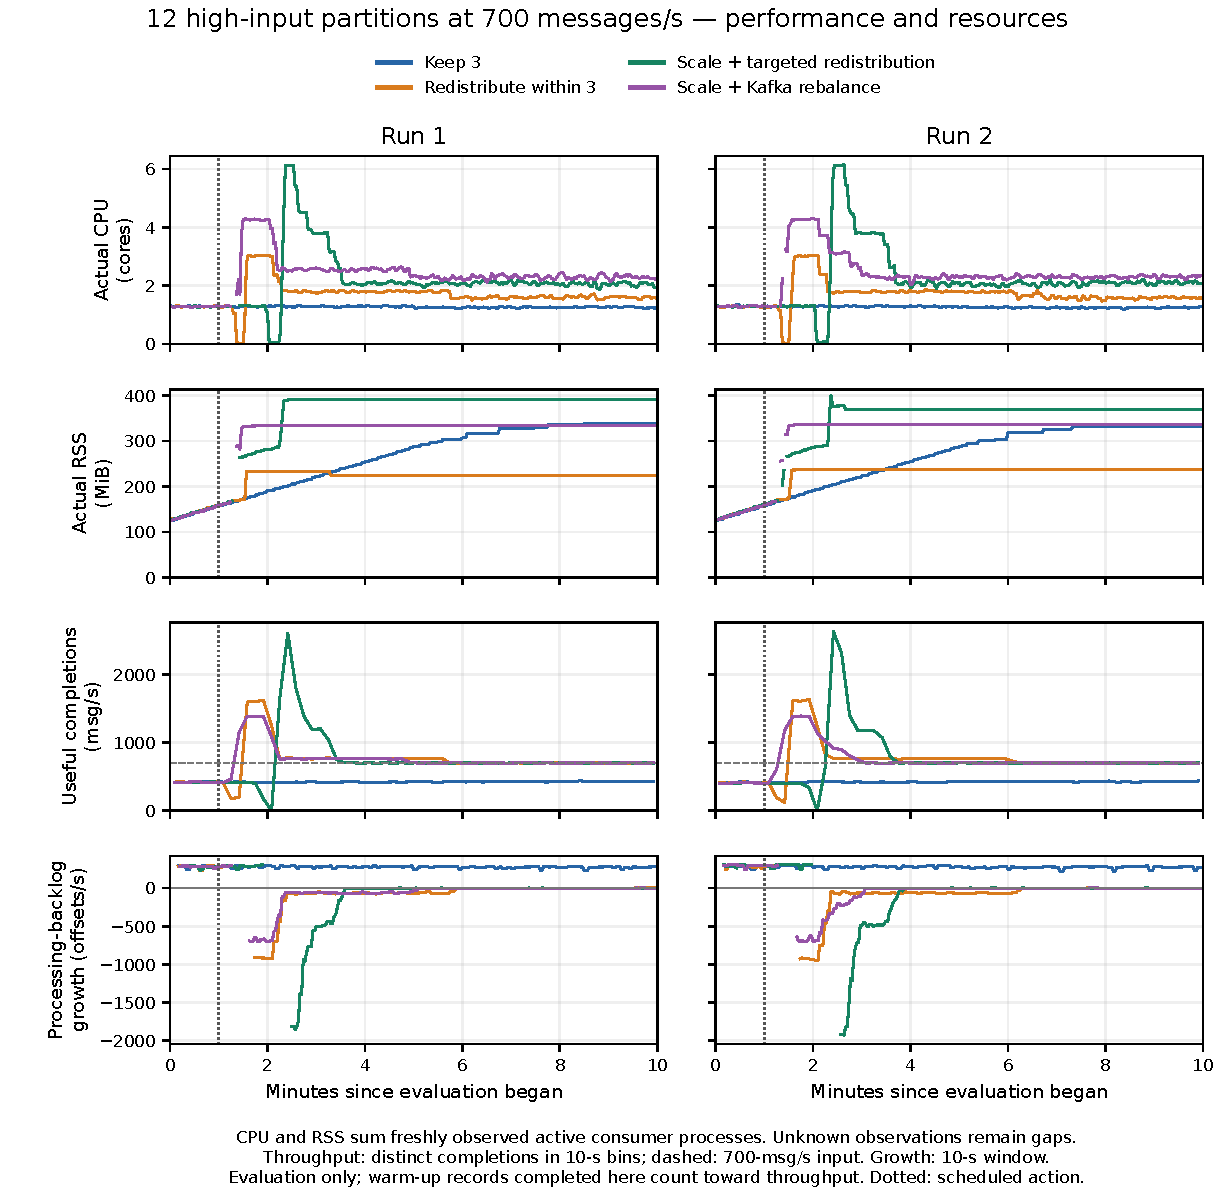
\includegraphics[width=\linewidth,height=.79\textheight,keepaspectratio]{figures/twelve-partition-compact-performance.pdf}
\caption{Actual consumer CPU and resident memory, useful completion throughput, and ten-second processing-backlog growth. Resource traces sum fresh measurements for all started consumer processes; an unavailable component leaves a gap. Requested resources and their integrals remain separate in the resource table.}
\label{fig:twelve-partition-compact-performance}
\end{figure}
\clearpage
\begin{figure}[p]
\centering
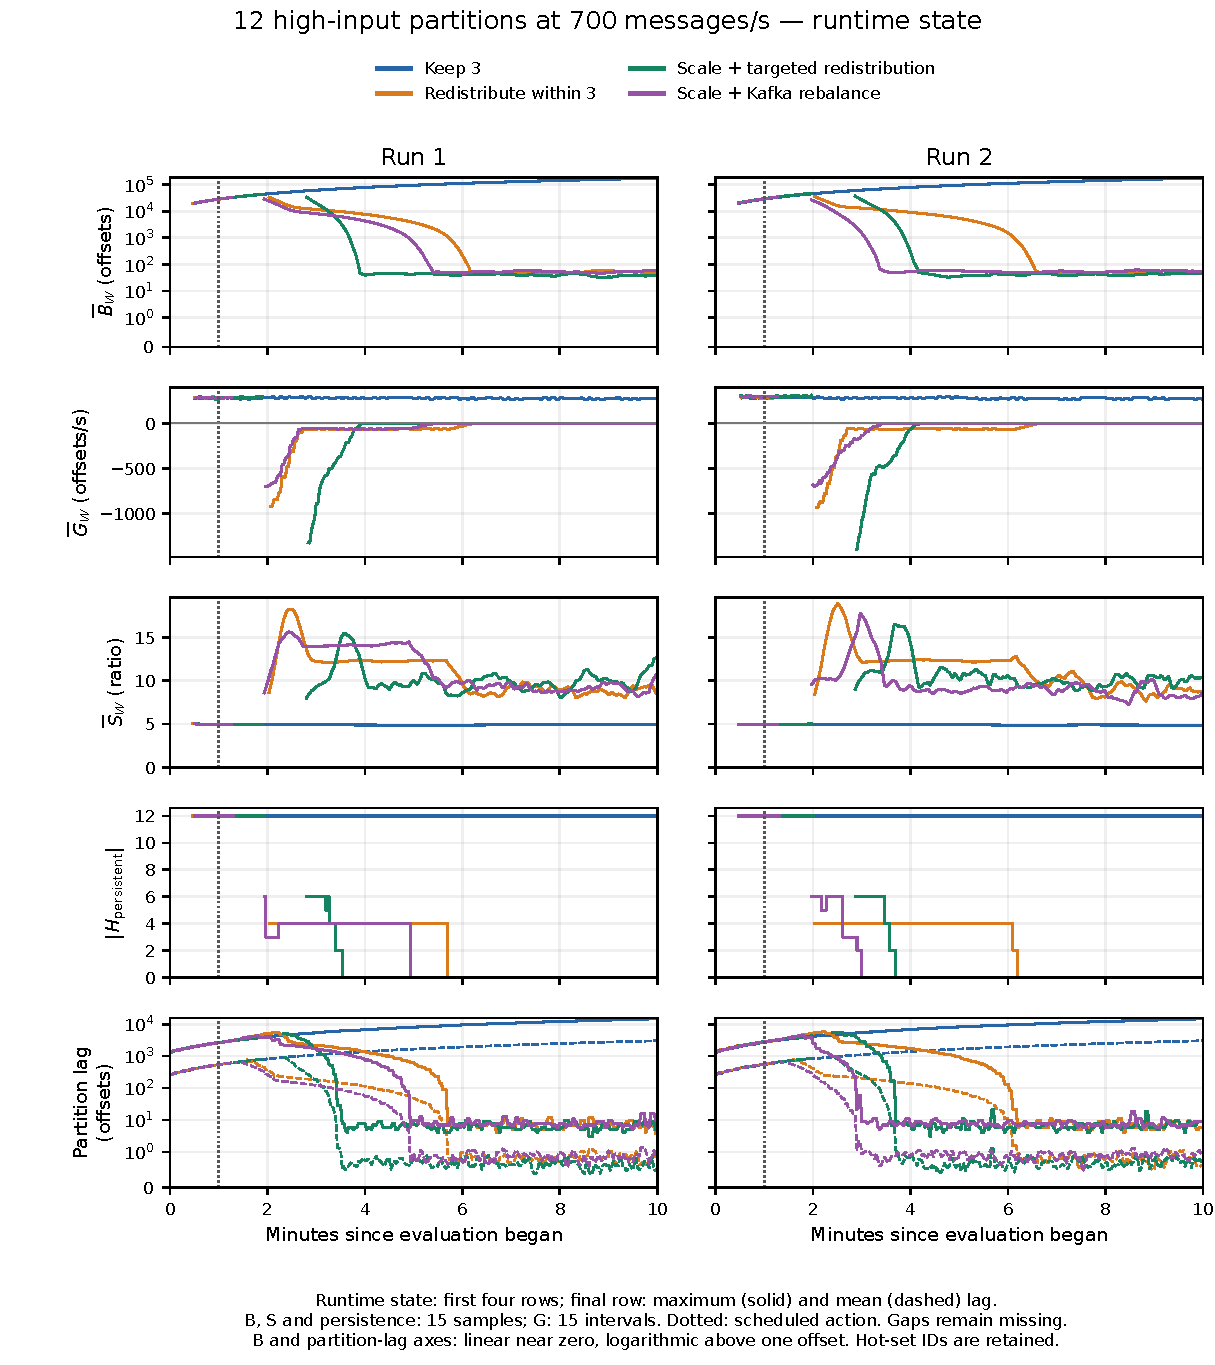
\includegraphics[width=\linewidth,height=.79\textheight,keepaspectratio]{figures/twelve-partition-runtime-state.pdf}
\caption{Reconstructed runtime state and partition-lag diagnostics. The first four rows show window-mean total lag, window growth, window-mean skew and persistent-hot count. The final row shows maximum and mean partition lag. Exact persistent-hot identifiers remain in the supporting data; the count alone does not identify a reassignment target. No scheduled action was selected by this reconstructed state.}
\label{fig:twelve-partition-runtime-state}
\end{figure}
\clearpage

\clearpage
\subsection{Four high-input partitions: ten-minute evaluation}\label{sec:four-partition-updated}
This follow-up kept the 700-message/s total input rate, but concentrated 80\% of the input on four of sixty partitions, initially owned by Consumer 2. The remaining partitions shared the other 20\%. Timing and processing settings matched the twelve-partition comparison. Redistribution within three consumers and scaling to six with targeted redistribution were each tested twice, using workload seeds 81 and 82 and reversing their order in the second repetition. Initial ownership and the original consumer placement were checked. Table~\ref{tab:combined-partition-ownership} gives the final assignments; this follow-up did not include normal Kafka scaling or a no-mitigation run.

Both responses completed all evaluation messages by the drain cutoff. Redistribution within three had lower p99, fewer one-second SLO violations, less backlog and lower resource use in both runs. It also caused shorter processing pauses and confirmed recovery sooner. Tables~\ref{tab:four-partition-outcomes}--\ref{tab:four-partition-intervention-cost} provide the values. Thus, adding consumers did not improve the tested outcomes for this workload. Six consumers retained the earlier scaling setting; this experiment did not establish an optimal consumer count.

For messages produced during the final two evaluation minutes, p99 was 0.187 and 0.349 seconds with redistribution, compared with 2.714 and 0.481 seconds with targeted scaling. All of these messages completed by the drain cutoff. This interval was specified before these trials, unlike the retrospective twelve-partition analysis. The first targeted-scaling run developed another backlog spike after meeting the recovery criterion, showing that an initial recovery does not guarantee continuously low backlog.

Small persistent-hot sets sometimes remained late in these runs despite low absolute backlog. The runtime-state figure therefore needs to be read alongside the absolute lag and growth measurements. Resource integrals use valid observations; per-process CPU coverage was 87.22--99.72\%, interpreted as in Section~\ref{sec:twelve-partition-updated}.

\clearpage
\begingroup
\makeatletter
\setlength{\@fptop}{0pt}
\setlength{\@fpsep}{12pt}
\setlength{\@fpbot}{0pt plus 1fil}
\makeatother
\begin{table}[!htbp]
\centering\small
\setlength{\tabcolsep}{3pt}
\renewcommand{\arraystretch}{1.12}
\begin{tabular}{@{}lrrrrrr@{}}
\toprule
Response & Run & \shortstack{Mean latency\\(s)} & \shortstack{p99\\(s)} & \shortstack{Unfinished\\(\%)} & \shortstack{SLO violations\\1 s (\%)} & \shortstack{Useful throughput\\(msg/s)}\\
\midrule
Redistribute 3 & 1 & 10.749 & 84.50 & 0.000 & 26.63 & 730.87\\
Redistribute 3 & 2 & 9.935 & 79.28 & 0.000 & 25.82 & 731.38\\
Targeted scale 6 & 1 & 19.330 & 110.19 & 0.000 & 35.23 & 730.89\\
Targeted scale 6 & 2 & 20.023 & 112.94 & 0.000 & 34.72 & 731.13\\
\bottomrule
\end{tabular}
\caption{Completion outcomes: four high-traffic partitions.}
\label{tab:four-partition-outcomes}\label{tab:four-partition-latency-details}
\end{table}
\begin{table}[!htbp]
\centering\small
\setlength{\tabcolsep}{3pt}
\renewcommand{\arraystretch}{1.12}
\begin{tabular}{@{}lrrrrr@{}}
\toprule
Response & Run & \shortstack{Actual CPU\\(core-s)} & \shortstack{Actual RSS\\(GiB-min)} & \shortstack{Requested CPU\\(core-min)} & \shortstack{Requested memory\\(GiB-min)}\\
\midrule
Redistribute 3 & 1 & 1,006.9 & 2.75 & 72.00 & 36.00\\
Redistribute 3 & 2 & 1,018.7 & 2.72 & 72.00 & 36.00\\
Targeted scale 6 & 1 & 1,301.6 & 4.09 & 136.83 & 68.42\\
Targeted scale 6 & 2 & 1,300.6 & 4.01 & 136.85 & 68.42\\
\bottomrule
\end{tabular}
\caption{Consumer resources: four high-traffic partitions.}
\label{tab:four-partition-resources}
\end{table}
\begin{table}[!htbp]
\centering\small
\setlength{\tabcolsep}{3pt}
\renewcommand{\arraystretch}{1.12}
\begin{tabular}{@{}lrrrrrr@{}}
\toprule
Response & Run & \shortstack{Mean total\\lag} & \shortstack{Maximum\\total backlog} & \shortstack{Lag coverage\\(\%)} & \shortstack{Maximum\\partition lag} & Mean skew\\
\midrule
Redistribute 3 & 1 & 7,296 & 50,879 & 96.3 & 13,509 & 20.56\\
Redistribute 3 & 2 & 6,994 & 50,157 & 97.0 & 12,258 & 20.88\\
Targeted scale 6 & 1 & 12,683 & 66,598 & 95.7 & 15,839 & 23.00\\
Targeted scale 6 & 2 & 12,740 & 70,217 & 95.0 & 16,277 & 22.72\\
\bottomrule
\end{tabular}
\caption{Backlog and lag skew: four high-traffic partitions.}
\label{tab:four-partition-diagnostics}
\end{table}

\begin{table}[!htbp]
\centering\small
\setlength{\tabcolsep}{3pt}
\renewcommand{\arraystretch}{1.12}
\begin{tabular}{@{}lrrrrrr@{}}
\toprule
Response & Run & \shortstack{Decision to\\active (s)} & \shortstack{Global gap\\(s)} & \shortstack{Extra pending\\during pause} & \shortstack{Net pending\\during transfer} & \shortstack{Recovery\\(s)}\\
\midrule
Redistribute 3 & 1 & 27.26 & 15.080 & 10,557 & 7,023 & 180.9\\
Redistribute 3 & 2 & 21.92 & 12.307 & 8,614 & 6,019 & 173.4\\
Targeted scale 6 & 1 & 78.52 & 19.881 & 13,918 & 4,678 & 290.5\\
Targeted scale 6 & 2 & 81.26 & 21.732 & 15,305 & 5,523 & 266.8\\
\bottomrule
\end{tabular}
\caption{Intervention time and recovery: four high-traffic partitions.}
\label{tab:four-partition-intervention-cost}
\end{table}
\clearpage
\begin{figure}[!htbp]
\centering
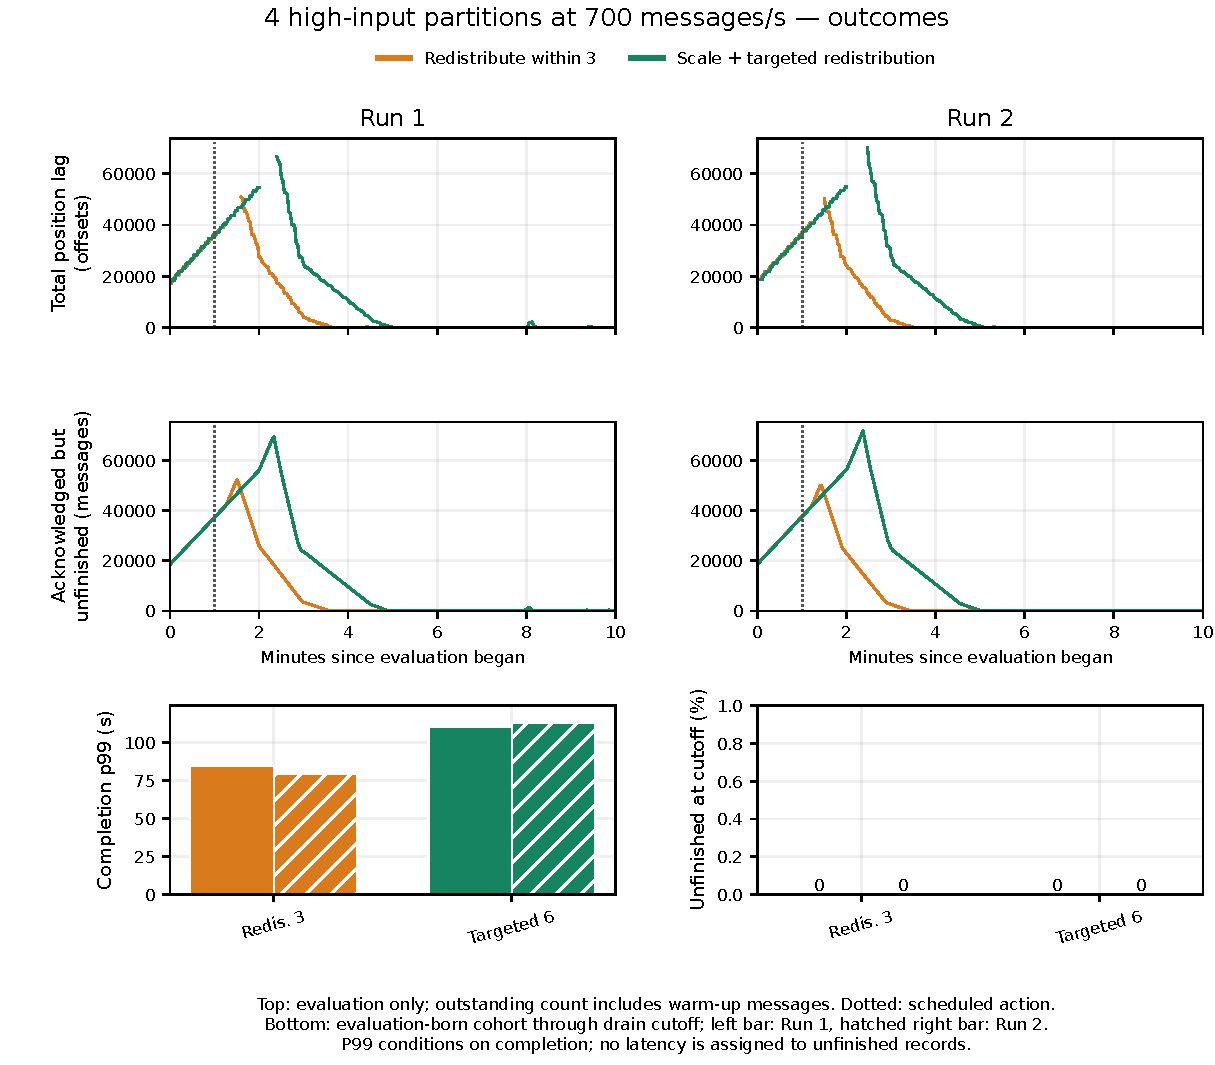
\includegraphics[width=\linewidth,height=.58\textheight,keepaspectratio]{figures/four-partition-compact-outcomes.pdf}
\caption{Outcomes with four high-traffic partitions. The upper panels show total consumer-position lag and acknowledged but unfinished messages during the ten-minute evaluation. The lower panels show p99 for completed evaluation messages and the unfinished percentage at the drain cutoff. Warm-up work is included in the time-series counts but excluded from the evaluation-message outcomes.}
\label{fig:four-partition-compact-outcomes}
\end{figure}
\clearpage

\begin{figure}[!htbp]
\centering
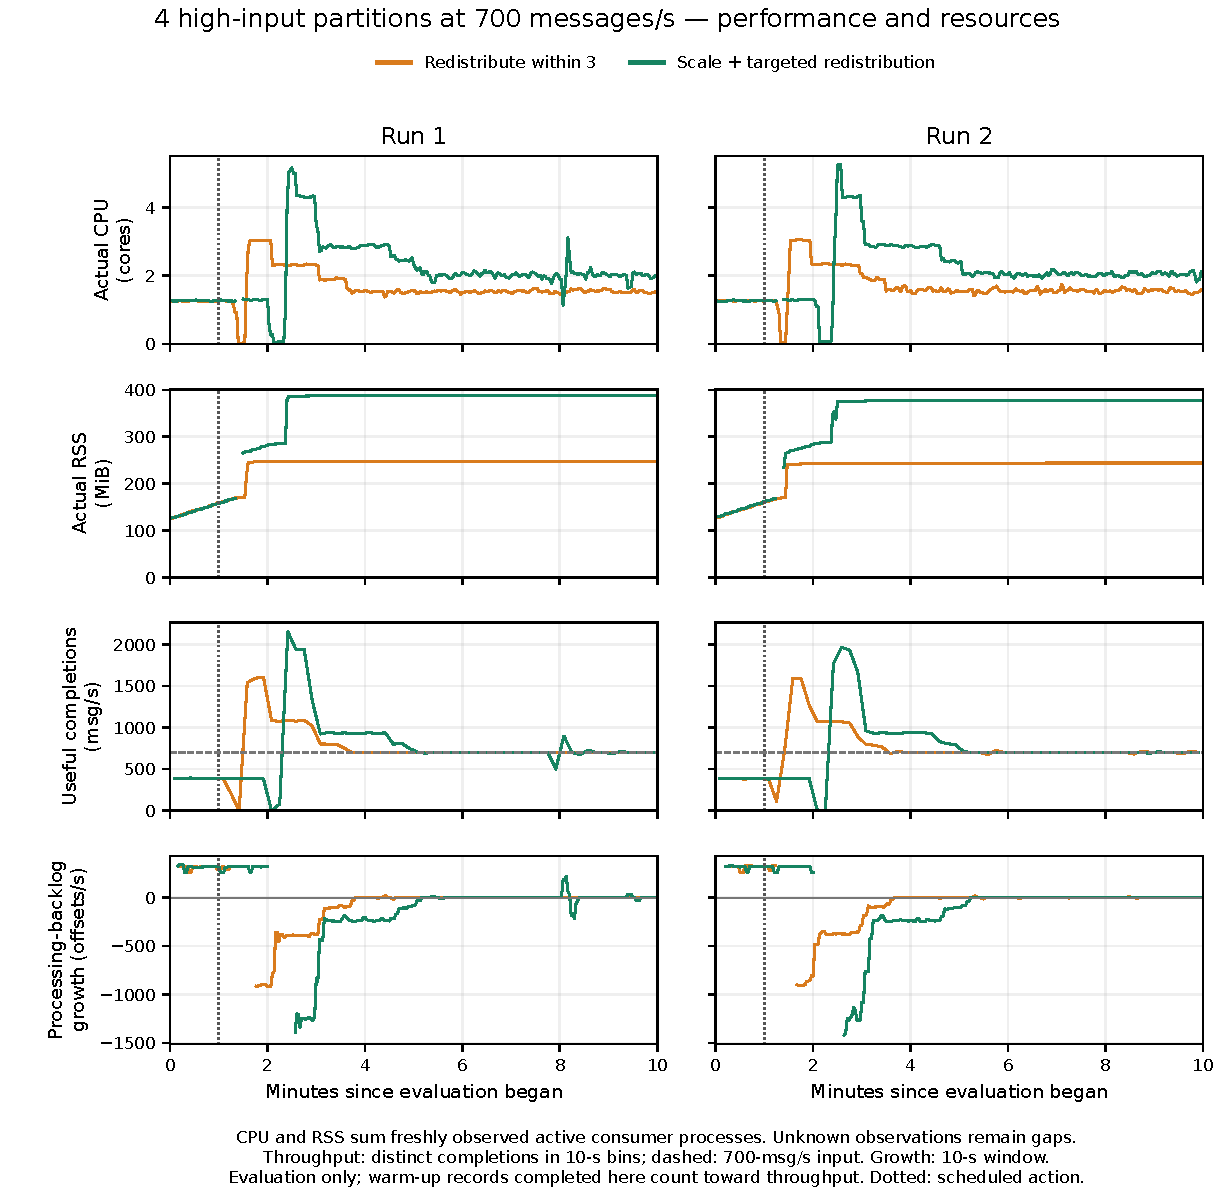
\includegraphics[width=\linewidth,height=.60\textheight,keepaspectratio]{figures/four-partition-compact-performance.pdf}
\caption{Consumer CPU use, resident memory, completion throughput and ten-second processing-backlog growth during the ten-minute evaluation. Resource traces sum fresh measurements for all started consumer processes; an unavailable component leaves a gap. Requested resources and their integrals remain separate in the resource table.}
\label{fig:four-partition-compact-performance}
\end{figure}
\clearpage
\begin{figure}[p]
\centering
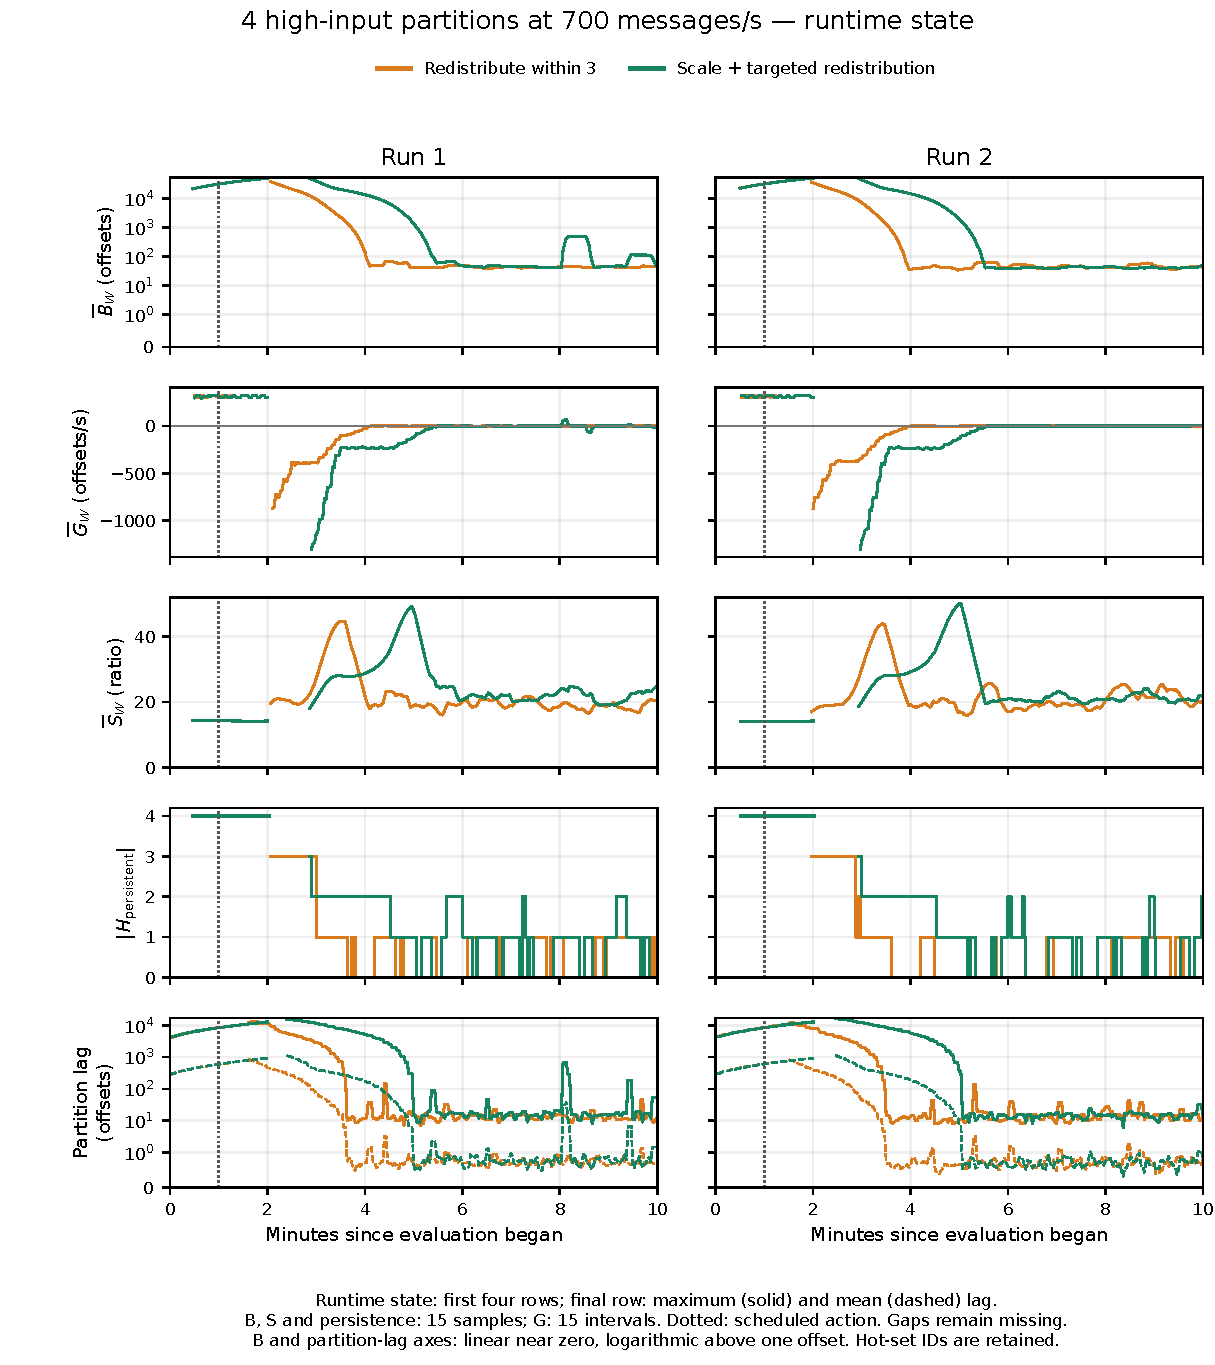
\includegraphics[width=\linewidth,height=.79\textheight,keepaspectratio]{figures/four-partition-runtime-state.pdf}
\caption{Partition-level measurements during the ten-minute evaluation. The first four rows show window-mean total lag, window growth, window-mean skew and persistent-hot count. The final row shows maximum and mean partition lag. Exact persistent-hot identifiers remain in the supporting data; the count alone does not identify a reassignment target. No scheduled action was selected by this reconstructed state.}
\label{fig:four-partition-runtime-state}
\end{figure}
\clearpage
\endgroup

\clearpage
\appendix
\section{Earlier five-minute experiments and sensitivity}
\subsection{Five-minute evaluation experiments: additional metrics}
These two earlier blocks each used a five-minute evaluation, one-minute warm-up and two-minute drain, with 210,000 admitted evaluation messages per trial. Each block contains its own unchanged-assignment baseline and its intervention, each run twice. They remain separate comparisons rather than being pooled into the later ten-minute experiments. Their diagnostics, process resources and retrospective completion-deadline sensitivity are included here for completeness.

The historical monitoring gaps are retained. Some predate the correction that initializes a returned-record position from a verified assignment offset while the client position remains unresolved. The correction was not applied retrospectively to invent missing values. Missing observations also restart the fifteen-observation persistence history, so the diagnostic gap may last longer than the ownership transfer itself. A shorter growth window cannot recover measurements that were never available. No comparison of these blocks with the later ten-minute blocks isolates duration alone: dates, selected partition identities and the monitoring implementation also changed.
\subsubsection{Five-minute evaluation: targeted scaling}
\begin{table}[!htbp]
\centering\small
\setlength{\tabcolsep}{3pt}
\renewcommand{\arraystretch}{1.12}
\begin{tabular}{@{}lrrrrr@{}}
\toprule
Response & Run & \shortstack{p99\\(s)} & \shortstack{Unfinished\\(\%)} & \shortstack{Misses $>1$ s\\(\%)} & \shortstack{Useful throughput\\(msg/s)}\\
\midrule
Keep 3 & 1 & 231.58 & 31.760 & 83.42 & 415.93\\
Targeted scale 6 & 1 & 110.70 & 0.000 & 57.01 & 757.32\\
Keep 3 & 2 & 229.28 & 31.037 & 83.24 & 418.90\\
Targeted scale 6 & 2 & 109.47 & 0.000 & 58.17 & 755.63\\
\bottomrule
\end{tabular}
\caption{Whole evaluation-born cohort through the fixed drain cutoff. Deadline misses include overdue unfinished messages. Useful throughput counts distinct completions during evaluation, including warm-up records completed then; it can exceed the input rate while queued work is cleared.}
\label{tab:short-targeted-scaling-outcomes}
\end{table}
\begin{table}[!htbp]
\centering\small
\setlength{\tabcolsep}{3pt}
\renewcommand{\arraystretch}{1.12}
\begin{tabular}{@{}lrrrrr@{}}
\toprule
Response & Run & \shortstack{Actual CPU\\(core-s)} & \shortstack{Actual RSS\\(GiB-min)} & \shortstack{Requested CPU\\(core-min)} & \shortstack{Requested memory\\(GiB-min)}\\
\midrule
Keep 3 & 1 & 515.3 & 1.57 & 42.00 & 21.00\\
Targeted scale 6 & 1 & 704.8 & 2.27 & 76.70 & 38.35\\
Keep 3 & 2 & 519.5 & 1.56 & --- & ---\\
Targeted scale 6 & 2 & 687.6 & 2.25 & 76.81 & 38.40\\
\bottomrule
\end{tabular}
\caption{Consumer resources over evaluation plus drain. Actual values integrate observed process CPU and RSS intervals and sum them across consumers. Requested values integrate Kubernetes resource declarations; neither is monetary or whole-cluster cost. A dash denotes unavailable full-window request coverage, not zero cost.}
\label{tab:short-targeted-scaling-resources}
\end{table}
\begin{table}[!htbp]
\centering\small
\setlength{\tabcolsep}{3pt}
\renewcommand{\arraystretch}{1.12}
\begin{tabular}{@{}lrrrrrr@{}}
\toprule
Response & Run & \shortstack{Mean total\\lag} & \shortstack{Peak total\\lag} & \shortstack{Lag coverage\\(\%)} & \shortstack{Peak partition\\lag} & Mean skew\\
\midrule
Keep 3 & 1 & 58,517 & 101,938 & 99.3 & 8,290 & 4.92\\
Targeted scale 6 & 1 & 19,438 & 50,671 & 86.0 & 4,960 & 8.47\\
Keep 3 & 2 & 57,077 & 99,351 & 99.3 & 8,047 & 4.93\\
Targeted scale 6 & 2 & 19,473 & 51,721 & 83.3 & 4,245 & 8.92\\
\bottomrule
\end{tabular}
\caption{Lag diagnostics during evaluation only, in offsets except skew and coverage. Means use trapezoidal area divided by covered time; peaks are sampled maxima. The time mean of the skew ratio is not the ratio of time-averaged maximum and mean lag. Invalid samples and ownership changes are not bridged.}
\label{tab:short-targeted-scaling-diagnostics}
\end{table}
\begin{figure}[p]
\centering
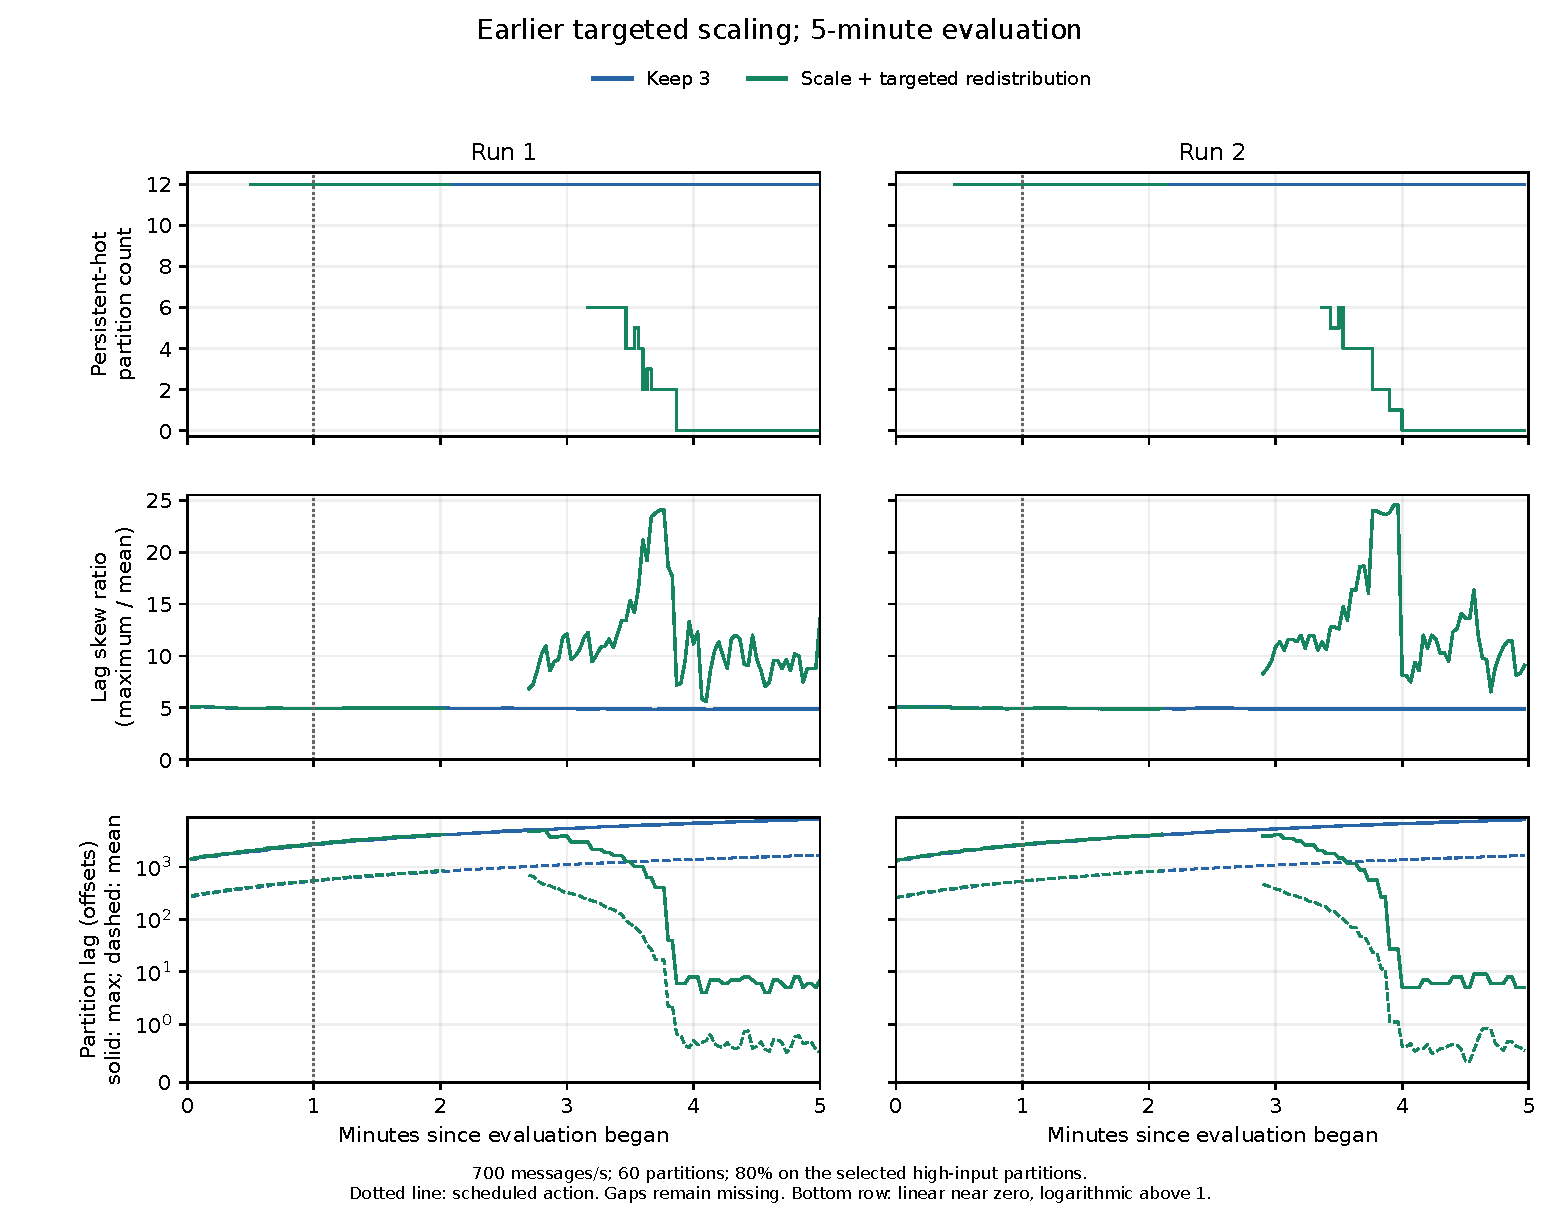
\includegraphics[width=\linewidth,height=.79\textheight,keepaspectratio]{figures/short-targeted-scaling-diagnostics.pdf}
\caption{Earlier five-minute evaluation with the original monitoring gaps retained. Persistent-hot counts, skew and maximum/mean partition lag are interpreted together.}
\label{fig:short-targeted-scaling-diagnostics}
\end{figure}
\clearpage
\subsubsection{Five-minute evaluation: redistribution}
\begin{table}[!htbp]
\centering\small
\setlength{\tabcolsep}{3pt}
\renewcommand{\arraystretch}{1.12}
\begin{tabular}{@{}lrrrrr@{}}
\toprule
Response & Run & \shortstack{p99\\(s)} & \shortstack{Unfinished\\(\%)} & \shortstack{Misses $>1$ s\\(\%)} & \shortstack{Useful throughput\\(msg/s)}\\
\midrule
Keep 3 & 1 & 226.34 & 30.182 & 83.41 & 422.08\\
Redistribute 3 & 1 & 103.76 & 0.000 & 61.59 & 725.25\\
Keep 3 & 2 & 227.13 & 30.475 & 83.24 & 421.76\\
Redistribute 3 & 2 & 91.38 & 0.000 & 60.84 & 727.54\\
\bottomrule
\end{tabular}
\caption{Whole evaluation-born cohort through the fixed drain cutoff. Deadline misses include overdue unfinished messages. Useful throughput counts distinct completions during evaluation, including warm-up records completed then; it can exceed the input rate while queued work is cleared.}
\label{tab:short-redistribution-outcomes}
\end{table}
\begin{table}[!htbp]
\centering\small
\setlength{\tabcolsep}{3pt}
\renewcommand{\arraystretch}{1.12}
\begin{tabular}{@{}lrrrrr@{}}
\toprule
Response & Run & \shortstack{Actual CPU\\(core-s)} & \shortstack{Actual RSS\\(GiB-min)} & \shortstack{Requested CPU\\(core-min)} & \shortstack{Requested memory\\(GiB-min)}\\
\midrule
Keep 3 & 1 & 515.8 & 1.56 & 42.00 & 21.00\\
Redistribute 3 & 1 & 554.1 & 1.47 & 42.00 & 21.00\\
Keep 3 & 2 & 516.5 & 1.55 & 42.00 & 21.00\\
Redistribute 3 & 2 & 553.4 & 1.46 & 42.00 & 21.00\\
\bottomrule
\end{tabular}
\caption{Consumer resources over evaluation plus drain. Actual values integrate observed process CPU and RSS intervals and sum them across consumers. Requested values integrate Kubernetes resource declarations; neither is monetary or whole-cluster cost. A dash denotes unavailable full-window request coverage, not zero cost.}
\label{tab:short-redistribution-resources}
\end{table}
\begin{table}[!htbp]
\centering\small
\setlength{\tabcolsep}{3pt}
\renewcommand{\arraystretch}{1.12}
\begin{tabular}{@{}lrrrrrr@{}}
\toprule
Response & Run & \shortstack{Mean total\\lag} & \shortstack{Peak total\\lag} & \shortstack{Lag coverage\\(\%)} & \shortstack{Peak partition\\lag} & Mean skew\\
\midrule
Keep 3 & 1 & 58,189 & 99,805 & 99.3 & 8,109 & 4.93\\
Redistribute 3 & 1 & 19,243 & 37,159 & 67.3 & 3,724 & 9.41\\
Keep 3 & 2 & 57,329 & 99,153 & 99.3 & 8,025 & 4.92\\
Redistribute 3 & 2 & 17,609 & 35,615 & 68.7 & 3,581 & 9.57\\
\bottomrule
\end{tabular}
\caption{Lag diagnostics during evaluation only, in offsets except skew and coverage. Means use trapezoidal area divided by covered time; peaks are sampled maxima. The time mean of the skew ratio is not the ratio of time-averaged maximum and mean lag. Invalid samples and ownership changes are not bridged.}
\label{tab:short-redistribution-diagnostics}
\end{table}
\begin{figure}[p]
\centering
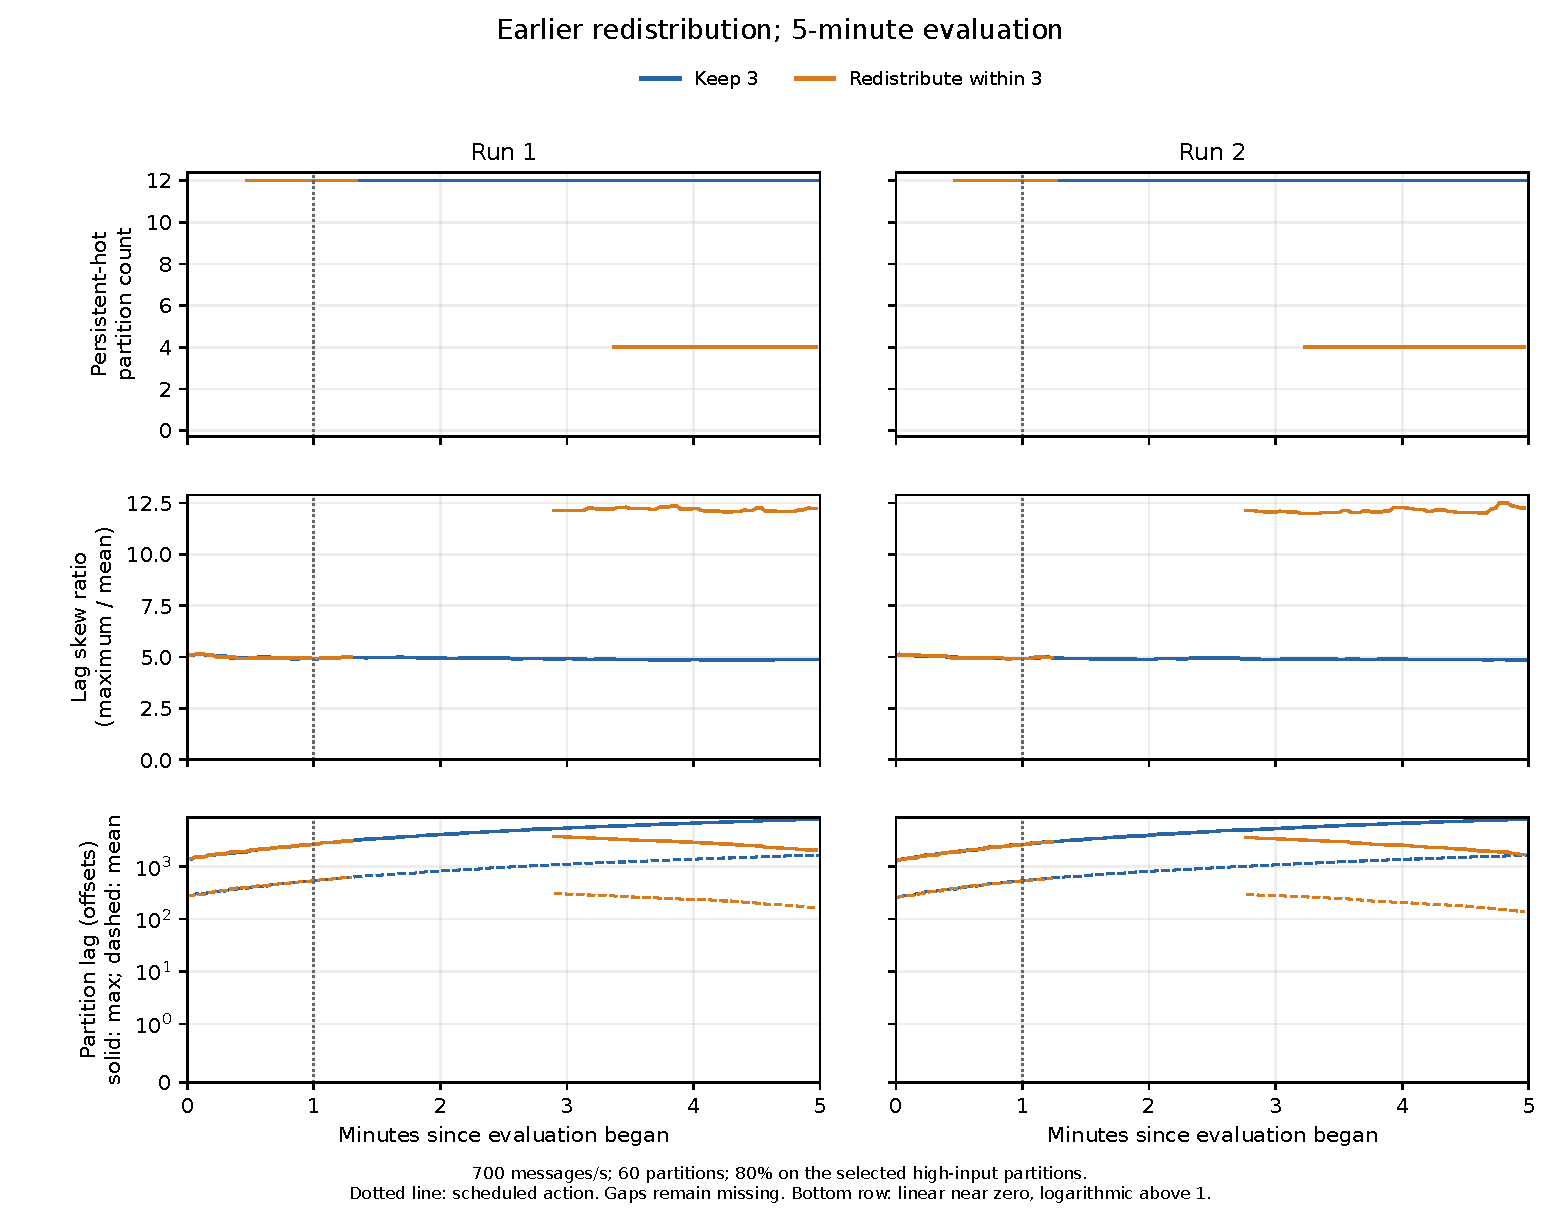
\includegraphics[width=\linewidth,height=.79\textheight,keepaspectratio]{figures/short-redistribution-diagnostics.pdf}
\caption{Earlier five-minute evaluation with the original monitoring gaps retained. Persistent-hot counts, skew and maximum/mean partition lag are interpreted together.}
\label{fig:short-redistribution-diagnostics}
\end{figure}
\clearpage

\clearpage
\subsection{Completion-deadline sensitivity}\label{app:deadline-sensitivity}
The half-second deadline is retained here to assess sensitivity. The main tables use one second. An overdue unfinished record is a miss at either applicable deadline; no unfinished latency is invented.
\begin{table}[!htbp]
\centering\small
\setlength{\tabcolsep}{3pt}
\renewcommand{\arraystretch}{1.12}
\begin{tabular}{@{}lrrr@{}}
\toprule
Response & Run & Misses $>0.5$ s (\%) & Misses $>1$ s (\%)\\
\midrule
Keep 3 & 1 & 83.336 & 83.321\\
Keep 3 & 2 & 83.388 & 83.364\\
Redistribute 3 & 1 & 30.705 & 30.496\\
Redistribute 3 & 2 & 32.200 & 31.838\\
Targeted scale 6 & 1 & 26.529 & 26.260\\
Targeted scale 6 & 2 & 27.586 & 27.331\\
Kafka scale 6 & 1 & 26.095 & 25.828\\
Kafka scale 6 & 2 & 21.255 & 21.051\\
\bottomrule
\end{tabular}
\caption{Twelve high-input partitions: ten-minute evaluation. Retrospective calculation; original 99-ms results remain preserved.}
\label{tab:twelve-partition-deadline-sensitivity}
\end{table}
\begin{table}[!htbp]
\centering\small
\setlength{\tabcolsep}{3pt}
\renewcommand{\arraystretch}{1.12}
\begin{tabular}{@{}lrrr@{}}
\toprule
Response & Run & Misses $>0.5$ s (\%) & Misses $>1$ s (\%)\\
\midrule
Redistribute 3 & 1 & 26.936 & 26.632\\
Redistribute 3 & 2 & 26.496 & 25.821\\
Targeted scale 6 & 1 & 36.053 & 35.232\\
Targeted scale 6 & 2 & 35.064 & 34.717\\
\bottomrule
\end{tabular}
\caption{Four high-input partitions: ten-minute evaluation. Both thresholds were prespecified.}
\label{tab:four-partition-deadline-sensitivity}
\end{table}
\begin{table}[!htbp]
\centering\small
\setlength{\tabcolsep}{3pt}
\renewcommand{\arraystretch}{1.12}
\begin{tabular}{@{}lrrr@{}}
\toprule
Response & Run & Misses $>0.5$ s (\%) & Misses $>1$ s (\%)\\
\midrule
Keep 3 & 1 & 83.447 & 83.418\\
Targeted scale 6 & 1 & 57.312 & 57.011\\
Keep 3 & 2 & 83.258 & 83.239\\
Targeted scale 6 & 2 & 58.572 & 58.171\\
\bottomrule
\end{tabular}
\caption{Five-minute evaluation: targeted scaling. Retrospective calculation; original 99-ms results remain preserved.}
\label{tab:short-targeted-scaling-deadline-sensitivity}
\end{table}
\begin{table}[!htbp]
\centering\small
\setlength{\tabcolsep}{3pt}
\renewcommand{\arraystretch}{1.12}
\begin{tabular}{@{}lrrr@{}}
\toprule
Response & Run & Misses $>0.5$ s (\%) & Misses $>1$ s (\%)\\
\midrule
Keep 3 & 1 & 83.438 & 83.413\\
Redistribute 3 & 1 & 61.794 & 61.591\\
Keep 3 & 2 & 83.278 & 83.241\\
Redistribute 3 & 2 & 61.100 & 60.840\\
\bottomrule
\end{tabular}
\caption{Five-minute evaluation: redistribution. Retrospective calculation; original 99-ms results remain preserved.}
\label{tab:short-redistribution-deadline-sensitivity}
\end{table}

\clearpage
\section{Measurement Coverage}
\label{app:measurement-coverage}
\begingroup
\centering\footnotesize
\setlength{\tabcolsep}{3pt}
\renewcommand{\arraystretch}{1.06}
\begin{longtable}{@{}>{\raggedright\arraybackslash}p{.22\linewidth}>{\raggedright\arraybackslash}p{.42\linewidth}>{\raggedright\arraybackslash}p{.29\linewidth}@{}}
\caption{Metric coverage and limitations.}
\label{tab:result-metric-coverage}\\
\toprule
Metric family & Evidence in results & Interpretation\\
\midrule\endfirsthead
\toprule
Metric family & Evidence in results & Interpretation\\\midrule\endhead
Partition lag and total lag & Main lag plots, diagnostic figure and lag-summary tables; older five-minute counterparts in the appendix. & Offsets, not guaranteed record counts.\\
Processing backlog and growth & Main backlog-growth plots and acknowledged-unfinished plots; growth is also retained for consumer-position lag. & Completion frontier and returned-record position have different definitions.\\
Maximum and mean partition lag & Bottom row of each diagnostic figure and tables of sampled maxima. & Maximum and mean are taken across partitions at each valid observation.\\
Lag skew and window-mean skew & Runtime-state row shows window-mean skew; the summary table and separate diagnostic plot retain raw skew. & High relative skew can coexist with small absolute lag.\\
Hot set, persistence score and persistent-hot set & Persistent-hot row, detector settings and interpretation of early versus late observations. & Exploratory diagnostic, not a validated controller trigger.\\
Window-mean backlog and runtime state & Runtime-state figure and timestamped CSV/JSON, including persistent-hot partition IDs. & Reconstructed from retained observations; no adaptive controller was evaluated.\\
Completion mean and p99 & Main outcome tables for each workload. & Calculated from completed evaluation messages through drain; p99 is not an average of rolling percentiles.\\
Unfinished work and completion deadlines & Unfinished percentage and 1-second cohort deadline misses in main tables; 0.5-second sensitivity in appendix. & Overdue unfinished messages count as misses; they have no fabricated completion latency.\\
Input rate and useful throughput & Main throughput plots and outcome tables; acknowledged input rate in the text. & Useful throughput counts each distinct completed message once.\\
Actual CPU and resident memory & Main process traces and observed resource integrals. & Consumer processes only; no full-cluster energy or monetary-cost claim.\\
Requested CPU and memory cost & Main resource tables, integrated over evaluation plus drain; detailed resource-cost figures retained with records. & Partial request coverage is unavailable for full-run comparison, not zero.\\
Interruption, transition backlog and recovery & Main intervention-cost tables, with operational endpoints identified. & Recovery is first threshold confirmation while input continues; not permanent stability.\\
Correctness and measurement quality & Identity reconciliation, handover validation, clock limitations and explicit coverage discussion. & Checks cover the completed stateless synthetic trials.\\
Controller overhead, splitting and state-transfer cost & Explicitly identified as unevaluated future measurements. & No adaptive controller, hot-key splitting or stateful transfer was evaluated in these trials.\\
\bottomrule
\end{longtable}
\endgroup

\end{document}
